\chapter{Introduction}
\section{The search problem}
The Binary Search is a classical algorithm used to efficiently locate a hidden target element in a linearly ordered set. To do so, the searcher repeatedly picks the median element of such set, performs a comparison operation and in constant time learns if the target was found and if not, whether the target is above or below the median (For example see Figure \ref{fig:binary-search-subarrays}).


\begin{figure}[ht]
\centering
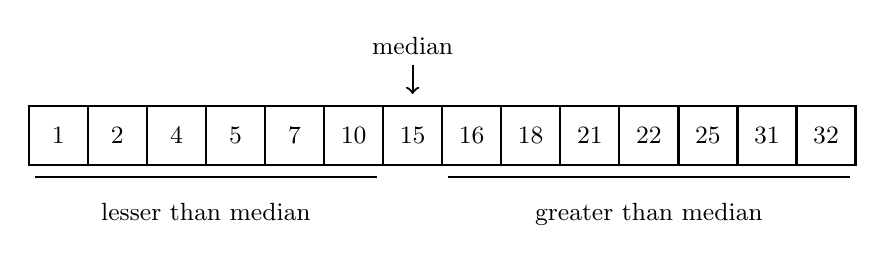
\begin{tikzpicture}[every node/.style={font=\small}, scale=0.75]

% --- Array values (10 elements) ---
\def\A{{1, 2, 4, 5, 7, 10, 15, 16, 18, 21, 22, 25, 31, 32}}
\def\MID{6} % Index of median (0-based): value = 23
% Draw array elements and indices
\foreach \i in {0,...,13} {
    \pgfmathsetmacro{\val}{\A[\i]}
    \draw[thick] (\i, 0) rectangle ++(1,1);
    \node at (\i+0.5, 0.5) {\val};
}

% Underline LEFT subarray (0..3)
\draw[thick] (0.1, -0.2) -- (6.0-0.1, -0.2);
% Label
\node[below=6pt] at (3, -0.2) {lesser than median};

% Underline RIGHT subarray (5..9)
\draw[thick] (7+0.1, -0.2) -- (13+1-0.1, -0.2);
% Label
\node[below=6pt] at (10.5, -0.2) {greater than median};

% Arrow for mid
\draw[<-, thick] (\MID+0.5, 1.2) -- +(0, 0.5) node[above] {median};

\end{tikzpicture}
\caption[Binary search]{Example of a sorted array containing 14 elements. }
\label{fig:binary-search-subarrays}
\end{figure}


The study of searching was initiated by D. Knuth in his seminal book \cite{Knuth1973} in which he discussed its various variants. However, the origins of the search problem reach the famous Rényi-Ulam game of twenty one questions in which a player is required to guess an unnamed object by asking yes-or-no questions\footnote{Note that in the twenty-one questions game one answer to a question may be a lie.}. Throughout the years, the searching and its variants have been continuously rediscovered under various definitions and names. This hints that the intuitions behind this problem resurface among multiple use cases and research domains. In fact, the search problem in its many variants is deeply connected with many other algorithmic notions including: parallelization of the Cholesky factorization, scheduling join operations in database queries, VLSI-layouts, learning theory, data clustering, graph cuts and parallel assembly of multi-part products. This work aims to serve as a survey of the results obtained for the problem and an experimental analysis of algorithms aimed at solving it.

The importance of searching is also due to its various practical applications. For example consider the following scenario: a complex procedure contains a hidden bug required to be fixed. The procedure is composed of multiple (often nested) blocks of code. In order to find this hidden bug the searcher can perform tests which allow him to check whether the given block of code contains the bug. After performing each such test they learn whether the bug is in or outside of the tested block. This process then continuous, until the bug is found. The problem is to find the best testing strategy for the tester in order to find the bug efficiently.

A different scenario may occur in the medical diagnostics. The so called \textit{House M.D. Problem} is concerned with diagnosing a potentially lethal, hidden disease. In order to do so, House and his medical team perform series of tests on the patient. These tests (often avant-garde in their nature) may include blood tests, a family survey or even breaking into the patients house. After performing each such test the team learns some new information about the patient which allows them to iteratively narrow the size of the space of possible diagnoses. The outcome of such test may include for example: the sugar level in blood is low (or high), the patients mother died of a disease with similar symptoms, the patient consumes very large amount of tuna etc. As the condition of the patient is deteriorating rapidly, the team needs to determine the disease as quickly as possible. 

\section{Problem statement}
\paragraph{Tree Search}
More formally, we model the search space as a tree $T$. The \textit{Vertex Tree Search Problem} is as follows: Among vertices of $T$ there is a hidden target vertex $x$ which is required to be located\footnote{It should be pointed out that the target vertex might not always be the same across multiple searches.}. During the search process, the searcher is allowed to perform queries, each about a chosen vertex $v\in V\br{T}$. In constant time the oracle responds whether the target is $v$ and if not, it identifies which connected component of $T-v$ contains $x$. Upon learning this information the searcher then iteratively picks the next vertex to query until the target is found. The goal is to create the optimal strategy for the searcher. 
One may also define an analogous process in which the queries concern edges. After a query to an edge $e$ the searcher learns which connected component of $T-e$ contains the target. We will call this problem the \textit{Edge Tree Search Problem}. For a visual example for both query models see Fig \ref{fig:sample_decision_trees_for_tree}.  

\begin{figure}[htbp]
    \centering
    \begin{minipage}{0.34\textwidth}
        \centering
        \tikz [tree layout, grow=-65,
               sibling distance=11mm, level distance=13mm,]
          \graph {
    ""[as=$a$] -- {
        ""[as=$b$] -- ""[as=$c$] -- {
            ""[as=$d$] -- ""[as=$e$],
            ""[as=$f$] -- { ""[as=$g$], ""[as=$h$], ""[as=$i$] }
        },
        ""[as=$j$] -- ""[as=$k$] -- { ""[as=$l$], ""[as=$m$] }
    }
};
    \caption[Sample tree]{}
    \label{fig:tree}
    \end{minipage}
    \begin{minipage}{0.32\textwidth}
        \centering
        \tikz [tree layout, grow=-90,
               sibling distance=12mm, level distance=14mm,]
          \graph {
            ""[as=$c$] -> { ""[as=$j$] -> { ""[as=$a$] -> ""[as=$b$],  ""[as=$l$] -> {""[as=$k$] -> ""[as=$m$]}}, ""[as=$h$] -> {""[as=$f$] -> {""[as=$g$], ""[as=$i$]}},  ""[as=$d$] -> ""[as=$e$]}
          };
    \caption[Vertex decision tree for a tree]{}
    \label{fig:dt_t_v}
    \end{minipage}
    \begin{minipage}{0.32\textwidth}
        \centering
        \tikz [tree layout, grow=-90,
               sibling distance=12mm, level distance=14mm,]
            \graph {
              ""[as=$aj$] -> {
                ""[as=$cf$] -> {""[as=$cd$] -> {""[as=$bc$], ""[as=$de$]},  ""[as=$fg$] -> ""[as=$fh$] -> ""[as=$fi$]]},
                ""[as=$km$] -> ""[as=$jk$] -> ""[as=$kl$]
              }
            };
        \caption[Edge decision tree for a tree]{}
        \label{fig:dt_t_e}
    \end{minipage}
        \caption[Tree and decision trees for it]{Sample input tree $T$ (Figure \ref{fig:tree}) and two decision trees for $T$: one for the Vertex Tree Search Problem (Figure \ref{fig:dt_t_v}) and one for the Edge Tree Search Problem (Figure \ref{fig:dt_t_e}).}
        \label{fig:sample_decision_trees_for_tree}
\end{figure}

When the input tree is a path both problems become the clasical binary search in the linearly ordered set.
We remark that for the vertex variant sometimes an alternative definition is provided. Upon query to $v$, if it is not the target, the response is an edge\footnote{Or equivaletly a vertex.} incident to $v$ which is the closest towards the target. This definition is equivalent as each component of $T-v$ has exactly one edge/vertex connecting it to $v$. A similar alternative/equivalent definition holds for the edge Tree Search Problem in which the response is the unique endpoint of $e$ laying closer to the target. The distinction between the two ways of defining the problem becomes significant when attempting to generalize it to arbitrary graphs.


\paragraph{Graph Search} In the following considerations we will be concerned with the generalization of the first definition of the Tree Search Problem. Given a graph $G$ the \textit{Vertex Graph Search Problem} is as follows: Among vertices of $G$ there exists a hidden target vertex $x$ which is required to be located. During the search process, the searcher is allowed to perform queries, each about a chosen vertex $v\in V\br{G}$. In constant time the oracle responds whether the target is $v$ and if not, it identifies which connected component of $G-v$ contains $x$. Again, the goal is to create the optimal strategy for the searcher. As before, a similar definition can be provided for the edge query model, which provides us with the \textit{Edge Graph Search Problem}. For a visual example of both query models see Figure \ref{fig:sample_decision_trees_for_graph}.

% In this generalized version of the problem, sometimes it might be the case that there is only one component $H\in G-v$. After a query to $v$, whenever $v$ is not the target the answer is always $H$. On the other hand, define the response to the query to $v$ as a vertex laying on the shortest path towards $x$. Whenever $v$ is not the target, there are exactly $\spr{N\br{v}}$ possible responses, Notice that in such case for each such response $u\in N(v)$ there is at least one vertex (namely the $u$ itself) for which the response is $u$ when it is the target. In fact the difference between the problems is also evident when considering their hardness. The "connected component" version of the problem is NP-hard while the "closest neighbor" version can be solved in quasipolynomial time. The choice of the generalization studied is a matter of taste, note that however the shortest distance query model may not behave deterministically. This is due to the fact that whenever there is more then one shortest path between $v$ and $x$ the answer to a query to $v$ may not always be the same. As this work deals only with the deterministic variants of the problem this choice arises naturally.


\begin{figure}[htbp]
    \centering
    \begin{minipage}{0.32\textwidth}
        \centering
        \tikz [node distance = 16mm, rotate=-90]
        \graph [spring layout]
{
  a -- { b, c, d, e};
  b -- {c};
  e -- {j, h};
  d -- {i, f};
  j -- {g[> orient=right]};
  i -- {j, e, k};
  g -- {l};
  h --  a;
  l -- {k};
};
        \caption[Sample graph and decision tree]{}
        \label{fig:graph}
    \end{minipage}
    \begin{minipage}{0.34\textwidth}
        \centering
        \tikz [tree layout, grow=-90,
               sibling distance=11mm, level distance=14.5mm,]
          \graph {
            ""[as=$e$] ->
            ""[as=$i$] -> { ""[as=$a$] -> { ""[as=$c$] -> ""[as=$b$],  ""[as=$h$],""[as=$f$] -> ""[as=$d$]}, ""[as=$g$] -> {""[as=$j$], ""[as=$k$] -> ""[as=$l$]}}
          };
        \caption[Vertex decision tree for a graph]{}
        \label{fig:dt_g_v}
    \end{minipage}
    \hfill
    \begin{minipage}{0.32\textwidth}
        \centering
        \tikz [tree layout, grow=-90,
               sibling distance=10, 
               level distance=8mm]
            \graph {
            ""[as=$ef$] -> 
            ""[as=$ei$] -> 
            ""[as=$ad$] -> {
                ""[as=$ae$] -> ""[as=$ac$] -> ""[as=$ah$] -> {""[as=$eh$], ""[as=$ab$] -> ""[as=$bc$]},
                ""[as=$ij$] -> ""[as=$ik$] -> {""[as=$di$] -> ""[as=$df$], ""[as=$kl$] -> ""[as=$gl$] -> ""[as=$gj$]}
              }
            };
    \caption[Edge decision tree for a graph]{}
    \label{fig:dt_g_e}
    \end{minipage}
        \caption[Graph and decision trees for it]{Sample input graph $G$ (Figure \ref{fig:graph}) and two decision trees for $G$: one for the Vertex Tree Graph Problem (Figure \ref{fig:dt_g_v}) and one for the Edge Graph Search Problem (Figure \ref{fig:dt_g_e}).}                  \label{fig:sample_decision_trees_for_graph}
\end{figure}
\paragraph{Poset Search and the Binary Identification Problem}
A different generalization of the Edge Tree Search Problem is the \textit{Poset Search Problem}. In this problem we are given a partially ordered set (poset) $\mathcal{P}=\br{X, \preceq}$, where $X$ denotes the ground set of objects and $\preceq$ is a partial ordering of elements of $X$. In order for the problem to be properly defined we also require that $\mathcal{P}$ contains a unique maximum element $r$. Among $X$ there is a unique hidden target element $x$ which is required to be located. During the search process, the searcher is allowed to perform queries asking whether $x\preceq v$ for a chosen $v\in X$. Once again, the goal is to create the optimal strategy for the searcher. For a visual example see Figure \ref{fig:sample_decision_tree_for_poset}.


\begin{figure}[htbp]
    \centering
    \begin{minipage}{0.48\textwidth}
        \centering
        \centering
        \tikz[rounded corners, <-, >=stealth % <--- strzałki w górę
]
\graph [
  layered layout,
  grow'=up, % <--- kluczowy element
  polyline layer edge routing,
  sibling distance=13mm,
  level distance=15mm
] {
  a <- { b, c, g };
  c <- i;
  b <- { d, e, f };
  d <- h;
  e <- h;
  f <- i;
  h <- m;
  g <- {j,k,l};
  j <- m;
  k <- m;
};
        \caption[Sample poset]{}
        \label{poset}
    \end{minipage}
    \hfill
    \begin{minipage}{0.48\textwidth}
        \centering
        \tikz [tree layout, grow=-90,
               sibling distance=15mm, level distance=12mm]
            \graph {
            ""[as=$b$] -> {
            ""[as=$e$] -> {""[as=$m$], ""[as=$f$] -> {""[as=$d$], ""[as=$i$]}}, ""[as=$g$] -> {""[as=$c$], ""[as=$j$] -> ""[as=$k$] -> ""[as=$l$]}}
            };
        \caption[Decision tree for a poset]{}
        \label{fig:dt_p}
    \end{minipage}
    \caption[Poset and a decision tree for it]{Sample poset $\mathcal{P}$ (Figure \ref{poset}) and a decision tree for it (Figure \ref{fig:dt_p}).}
    \label{fig:sample_decision_tree_for_poset}
\end{figure}

The Poset Search Problem can be generalized even further by allowing each available query to be any partition of the search space. In the \textit{Binary Identification Problem} we are given a pair $\br{\mathcal{H}, \mathcal{Q}}$ where $\mathcal{H}$ is a set of hypotheses and $\mathcal{Q}$ is a set of queries. Each query $q = \brc{R_1, R_2,...R_k}$ is a partition of $\mathcal{H}$ (we require that $\bigcup_{R\in q}R=\mathcal{H}$ and for any $R_1,R_2\in q$: $R_1\cap R_2=\emptyset$). After performing a chosen query the searcher obtains information which $R\in q$ contains the hidden target. This process continuous iteratively until the target if found. For a visual example see Figure \ref{fig:sample_decision_tree_binary_identification_problem}. 

In this broad sense this general model of searching can be interpreted using the information theory point of view. There exists a unique true hypotheses $h$ among the set $H=\brc{h_1,...,h_n}$ which the learner is trying to obtain. In order to do so, they iteratively collect small pieces of information which allow them to rule out certain hypothesis narrowing the search space. They do so until there is only one such hypothesis left. Analogously, the goal is to design a learning strategy which enables an efficient obtaining of this hidden hypothesis. 


\begin{figure}[htbp]
    \centering
    \begin{minipage}{0.48\textwidth}
        \centering
        \begin{tabular}{|c|c|c|c|c|c|c|c|c|c|}
\hline
 & $q_1$ & $q_2$ & $q_3$ & $q_4$ & $q_5$ & $q_6$ & $q_7$ & $q_8$ & $q_9$\\
\hline
$a$ & 1 & 2 & 1 & 1 & 1 & 1 & 1 & 1 & 1 \\
\hline
$b$ & 1 & 1 & 1 & 1 & 2 & 2 & 1 & 1 & 1 \\
\hline
$c$ & 1 & 3 & 1 & 1 & 3 & 3 & 1 & 2 & 1 \\
\hline
$d$ & 1 & 3 & 2 & 1 & 3 & 1 & 1 & 2 & 1 \\
\hline
$e$ & 2 & 1 & 2 & 2 & 1 & 2 & 1 & 2 & 1 \\
\hline
$f$ & 2 & 2 & 2 & 1 & 1 & 1 & 1 & 2 & 1 \\
\hline
$g$ & 2 & 1 & 2 & 1 & 1 & 2 & 2 & 2 & 1 \\
\hline
$h$ & 2 & 1 & 2 & 3 & 2 & 3 & 1 & 2 & 1 \\
\hline
$i$ & 2 & 1 & 2 & 1 & 2 & 3 & 1 & 2 & 2 \\
\hline
$j$ & 2 & 1 & 2 & 1 & 2 & 2 & 2 & 2 & 2 \\
\hline
$k$ & 2 & 1 & 2 & 4 & 2 & 2 & 2 & 2 & 2 \\
\hline
\end{tabular}
        \caption[Sample Binary Identification Problem instance]{}
        \label{bip}
    \end{minipage}
    \hfill
    \begin{minipage}{0.48\textwidth}
        \centering
        \tikz [tree layout, grow=-90,
               sibling distance=14mm, level distance=9.5mm]
            \graph {
            ""[as=$q_8$] -> {""[as=$q_6$], ""[as=$q_9$] -> {""[as=$q_1$] -> {""[as=$q_3$], ""[as=$q_5$] -> {""[as=$q_2$] -> ""[as=$q_7$]}},""[as=$q_6$] -> {""[as=$q_4$]}}}
            };
        \caption[Decision tree for Binary Identification Problem instance]{}
        \label{fig:dt_bip}
    \end{minipage}
    \caption[Sample Binary Identification Problem instance and Decision Tree for it]{Sample Binary Identification Problem instance (Figure \ref{bip}) and a decision tree for it (Figure \ref{fig:dt_bip}).}
    \label{fig:sample_decision_tree_binary_identification_problem}
\end{figure}

\paragraph{Strategies, Decision Trees and their costs}
Notice, that while defining the searching the term strategy was never properly defined. The \textit{search strategy} is an adaptive algorithm which (in polynomial time) provides the searcher with the next query to perform (given the previous responses). A natural way to visualize such strategy is to see it as a decision tree. A \textit{decision tree} $D$ is a rooted tree in which each vertex represents a query and each edge represents a possible response. The search is conducted by choosing as the next query the root of $D$. After receiving the response (If the search is not terminated) the searcher moves along the edge $e=(r, r_e)$ incident to $r$ associated with the response. The process then recurses in $D_{r_e}$ until the target is found. It should be noted however, that this is far from the only viable way of encoding the search strategy. The choice of the data structure used is a matter of taste and often leads to simpler design and analysis of the algorithms.

In order to sensibly talk about the quality of such strategy we need to also measure its cost. The cost of locating a vertex $x$ using a strategy $A$ is the amount of queries required to be performed to find $x$ using $\mathcal{A}$. The two most intuitive ways to measure the overall cost of $\mathcal{A}$ are: 
\begin{itemize}
    \item The worst case search time which is maximum of costs of $\mathcal{A}$ over all vertices
    \item The average case which is the sum of costs of $\mathcal{A}$ over all vertices\footnote{The average of and the sum are equivalent up to a constant factor of $n$.}.
\end{itemize}

Even though similar, these two criterion often differ in their analysis and algorithms constructed for them usually exploit slightly different properties of the input. It is often the case that greedy heuristics perform much better when we measure the average case cost of the decision trees created by them. In contrast, in the worst case, often the best known solutions require some intricate dynamic programming procedure as an essential subroutine. Interestingly enough, it is not hard to show that given two decision trees: one with good performance in the average case and one with good performance in the worst case, a simple algorithm can be used to create new decision tree with fairly good performance in both metrics \cite{Tradingoff}.

\paragraph{Weights and Costs}
Above, we have made the assumption that performing each query costs us exactly the same. In real life applications it might not be a case. For example, determining the value of some complex comparison operation for two large objects may take a substantial amount of time. In such cases we associate with each query a cost function. To calculate the cost of finding $x$, instead of measuring the amount of queries, we measure the sum of their costs. The worst case and the average case criteria are then defined according to this new values. 

Additionally, when dealing with the average case version of the problem, one may consider a scenario in which certain vertices are searched for more often then the others. In general, we can associate with each vertex a probability/frequency of it being searched for which we will call its weight. In this case the average query time naturally becomes the weighted average according to this weight function \footnote{We assume that these cost and weight functions are known \textit{a-priori}.}.
\section{The three field notation for the search problem}
One may see that the multiplicity of variants for the problem have started to be somewhat problematic. Ideally, we would like to introduce some unified way of speaking about the problem to avoid ambiguity. This is problematic because historically, various variants of the problem were often explored independently. To alleviate this inconvenience we introduce the following three field notation resembling the notation commonly used in task scheduling problems. Similarly, our notation will consists of the three following fields: $\alpha, \beta$ and $\gamma$. The $\alpha$ field is the search space environment field resembling the machine environment. The $\beta$ field is the query characteristics which resembles the job characteristics. The $\gamma$ field is the objective function which we are trying to optimize. In order not to confuse these two notations in contrary to single line separator used in scheduling ($\alpha|\beta|\gamma$), we will separate the three fields with doubled lines: $\alpha||\beta||\gamma$. The following table showcases example variants which may be considered:

\begin{table}[ht]
\centering
\begin{tabularx}{\textwidth}{|X|X|X|}
\hline
\text{$\alpha$ - search space } & \text{$\beta$ - query characteristics } & \text{$\gamma$ - objective value} \\
\hline
$P$ - paths
\newline
$T$ - trees
\newline
$POSET$ - POSETs
\newline 
$G$ - graphs
\newline
$HT$ - hypertrees
\newline
$HG$ - hypergraphs
\newline
$S$ - any set of hypothesis
& 
$E$ - edge queries
\newline
$V$ - vertex queries
\newline
$Q$ - any queries
\newline
$c$ - cost function on queries
\newline
$w$ - weight function on vertices
\newline
$d$ - due dates
\newline
$\Bar{d}$ - strict deadlines
\newline
$r$ - release times
\newline
$prec$ - precedences
& 
$C_{max}$ - maximum search time
\newline
$\sum C_i$ - average search time
\newline
$\sum U_i$ - throughtput
\newline
$F_{max}$ - maximum flow time
\newline
$\sum F_i$ - average flow time
\newline
$L_{max}$ - maximum lateness
\newline
$\sum L_i$ - average lateness
\newline
$T_{max}$ - maximum tardiness
\newline
$\sum T_i$ - average tardiness
\\
\hline
\end{tabularx}
\caption{Sample values for the three field notation for the search problem.}
\end{table}

The striking resemblance between these two notations suggests that we can view the search problem as a specific form of scheduling, in which the search strategy is the schedule and the queries are the jobs. From the perspective of the researcher however, the search problem is not nearly as explored as the scheduling problems and most of the variants which can be constructed using the table above are not even mentioned in the literature. It also seems, that the search problem is in a sense harder than the usual scheduling. For example, the best algorithm\footnote{This algorithm is obtained by a recursive usage of a QPTAS obtained via a non-trivial dynamic programming procedure. For details see: [insert ref here].} known for the NP-hard variant $T||V, c||C_{max}$ achieves an $O\br{\sqrt{\log n}}$-approximation \cite{dereniowski2017ApproxSsForGeneralBSinWTs}. A somewhat similar scheduling problem $P||C_{max}$ has a simple $\frac{4}{3}$-approximation algorithm based on sorting the jobs according to their costs \cite{BoundsonMultiprocessingTimingAnomalies}, admits a PTAS for an unbounded number of machines \cite{Binpackingwithrestrictedpiecesizes} and if the number of machines is bounded an FPTAS can be obtained \cite{AlgorithmsforSchedulingIndependentTasks}.

\section{Many names, one problem}

As mentioned above, the search problem has been continuously rediscovered under various names and definitions. It is usually the case, that each of these definitions is equivalent when the search space is a tree. The following list consists of different formulations under which the problem have been studied in the context of graphs: 
\begin{itemize}
    \item Binary Search \cite{OnakParys2006GenOfBSSInTsAndFLikePosets, dereniowski2017ApproxSsForGeneralBSinWTs, Deligkas2019BsInGsRev, Emamjomeh2016DetAndProbBSinGs, dereniowski2022CFApproxAlgForBSInTsWithMonoQTimes, dereniowski2024SInTsMonoQTs, noisyBSSFC, Dereniowski2024OnMG, EfficientNoisyBinarySearch, Dereniowski2023Edge},
    \item Tree Search Problem \cite{Jacobs2010OnTheComplexSearchInTsAvg, Cicalese2014ImprovedApproxAvgTs, Cicalese2016OnTSPwNonUniCost}, 
    \item Binary Identification Problem \cite{Cicalese2012BinIdentPForWTs, Karbasi2013Constrained}, 
    \item Ranking Colorings \cite{Knuth1973, Dereniowski2009ERankOfWTs, DereniowskiERAndSInPOSets, DereniowskiEfPQProcByGRank, DereniowskiVxRankOfChGsAndWTs, Lam1998ERankOfGsIsH}, 
    \item Ordered Colorings \cite{KATCHALSKI1995141}, 
    \item Elimination Trees \cite{Pothen1988OptimalEliminationTrees}, 
    \item Hub Labeling \cite{Angelidakis2018ShortestPQ},
    \item Tree-Depth \cite{NESETRIL20061022, BOROWIECKI2023113682},
    \item Partition Trees \cite{OnDasHC, Hgemo2024TightAB},
    \item Hierarchical Clustering \cite{Approximatehierarchicalclusteringviasparsestcutandspreadingmetrics}, 
    \item Search Trees on Trees \cite{SplayTonT, Fast_app_centroid_trees}, 
    \item LIFO-Search \cite{GIANNOPOULOU20122089}. 
\end{itemize}
Various different problem definitions stem from the learning theory including:
\begin{itemize}
    \item Decision Tree \cite{LABER2004209,ATightAnalysisofGreedy, GuptasApproxAlgsForOptDTsAndAdaptTSPPs, Tradingoff},
    \item Bayesian Active Learning \cite{NearoptimalBayesianactivelearning,Analysisofgreedyactivelearningstrategy},
    \item Discrete Function evaluation \cite{Diagnosisdetermination},
    \item Tree Split \cite{OnanOptimalSplitTreeProblem},
    \item Query Selection \cite{QuerySelection}.
\end{itemize}

Each of these problems is equivalent when restricted to trees, however for arbitrary graphs/search spaces this might not be the case. For example, in the generalized binary search problem in graphs (by convention) the response to the query to $v$ is the neighbor of $v$ laying on the shortest path towards the target. In contrast, in the Hierarchical Clustering the response to such query is the connected component of $T-v$ containing the target.
 
Among ambiguities resulting form the multiplicity of the problem definitions is the interpretation of the notion of weight. When considering the worst case cost, usually the weight is interpreted as the cost of a query. On the other hand, while analyzing the average case cost, the weight is usually the probability that the vertex will be searched for. In such scenario, the cost of the query (if present) is usually called cost. In this work we follow the second convention and we usually denote them as $w(v)$ and $c(v)$ (or $c(e)$ in edge query model) accordingly.

\section{The aim of the thesis}

Hereby, we will be mostly concerned with the situation in which the input graph is tree. A motivation for this is twofold. Firstly, trees come up most often in the practical scenarios regarding the problem. Secondly, from the algorithmic perspective, the most interesting and structural results are obtained for trees. Beyond that, most of the algorithms with provable guarantees follow some simple greedy rule and the achieved approximations are far from the objective value. For example, the problem $T||V||C_{max}$ is solvable in linear time (the algorithm is non-trivial)\cite{Schaffer1989OptNodeRankOfTsInLinTime}. If we however allow arbitrary graphs ($G||V||C_{max}$) then the problem becomes NP-hard even in chordal graphs \cite{DereniowskiVxRankOfChGsAndWTs} and the best known approximation in general case is $O\br{\log^{\frac{3}{2}} n }$ which is trivially obtained via an almost blackbox use of the tree decomposition of the graph \cite{RankingsofGraphs}. 

We conclude a series of experiments aimed at verifying whether the theoretical claims regarding the discussed algorithms are reflected in an experimental setup. In particular, we employ randomized techniques to generate various classes of inputs and test the performance of the implemented algorithms both in terms of running time and the quality of the solutions obtained.
\section{Organization of the work}
The second chapter serves as a more formal and detailed introduction necessary for further considerations. We formally restate all of the search models we are interested in and we recall the basic notions of graph theory required for the analysis.

The main part of the thesis is partitioned into two main chapters:

In the third chapter we focus ourselves on the formal analysis of the considered variants including the presentation of the most interesting algorithmic results for the problem. We showcase exact and approximation algorithms and few hardness results for the most complex variants of the search problem. 

The fourth chapter is a description of the computer experiments conducted in order to verify the theoretical claims regarding the performance of the previously presented algorithms.

The fifth chapter serves as a summary of our considerations and points the further research directions regarding this field.

